\documentclass[10pt]{article}\usepackage[correction,nu]{esial}
%\documentclass[10pt]{article}\usepackage[nu]{esial}
\usepackage{amstext,amsmath,amsfonts}
\TOP\unA
\newcommand{\WP}[1]{\textbf{WP}($#1$)}

\usepackage{amsthm,pifont,textcomp}
\usepackage{amsmath,amssymb}

\usepackage[utf8]{inputenc}
\graphicspath{{fig/}}

\begin{document}
\title{Examen du 19/03/2011 (2h)}
\fvset{fontsize=\footnotesize}
\maketitle

\begin{centering}
  \textbf{\large Documents interdits, à l'exception d'une feuille A4 à rendre
    avec votre copie.}

\end{centering}
\centerline{La notation tiendra compte de la présentation et de la clarté de
  la rédaction.}
\bigskip



\bigskip\QuestionCours~(2pt)

\Question(\textonehalf pt) Définissez en français (sans équation) les notations
$O$, $\Omega$ et $\Theta$ utilisées pour dénoter la complexité algorithmique en
insistant sur leurs relations les unes avec les autres.

\Question(\textonehalf pt) Quel est le rapport entre les notations que vous venez de définir et
les temps de calcul dans le meilleur des cas, le pire des cas et le cas moyen? 

\Question(\textonehalf pt) Définissez les tests (1) white box (2) de régression.

\begin{Reponse}
  \begin{itemize}
  \item \textbf{Whitebox:} C'est une technique de tests, une façon d'imaginer
    les tests à faire pour remplir mes objectifs; J'écris mes tests en lisant
    le source (et je teste donc les cas limites de l'implémentation)
  \item \textbf{Régression:} Quand j'ai trouvé une erreur (un bug) dans mon
    programme, je dois écrire un test cherchant à le reproduire afin de
    m'assurer que ce bug ne refera pas surface lors d'une modification
    ultérieure du code. 
  \end{itemize}
\end{Reponse}

\Question(\textonehalf pt) Définissez en quelques mots le principe des tris (1)
par insertion (2) par sélection en explicitant en français (sans équation)
leurs invariants.

\Exercice\textbf{Backtracking pour «Des chiffres et des lettres»} (D'après Eugène
Asarin -- 5pts)

Étant donné un tableau de lettres, on cherche à trouver le mot le plus long
composé de certaines de ces lettres. On s'interdit également d'utiliser les
lettres du tableau plus d'une fois. Par exemple, pour
\texttt{lettres=ERUIGHURH} le mot le plus long est RIGUEUR.

On suppose donné un objet dictionnaire \texttt{dict} doté d'une méthode
booléenne \texttt{contains(w)} qui répond si la chaîne \texttt{w} est un mot
valide du dictionnaire.

\Question(2pt) Programmez en Java une fonction récursive répondant au prototype
suivant, et qui renvoie un mot de $k$ lettres du dictionnaire, composé du
préfixe passé en paramètre et suivi de lettres du tableau utilisées au plus une
fois chacune. Si plusieurs mots répondant à cette définition existent, renvoyez
le premier d'entre eux que vous calculez. \\ 
\centerline{\framebox{\texttt{String chercher(String prefixe, char[] lettres,
      int k)}}}

Vous pouvez supposer que la proposition \texttt{lettres.length>k} est
vraie. \texttt{chercher(PA,"SETATTAH",7)} pourrait par exemple renvoyer
«PATATES». Si un tel mot n'existe pas il faut renvoyer \texttt{null}.\\
\textit{Indications:} Cette fonction est de complexité exponentielle; aucun mot
ne contient la lettre '*', qui peut donc être utilisée comme marqueur
temporaire.

\begin{Reponse}
  Le remplissage du dictionnaire est tout à fait améliorable :)

  \VerbatimInput{Mot.java}
\end{Reponse}

\Question(1pt) En utilisant cette fonction \texttt{chercher()}, écrivez la
fonction \texttt{jouer()} qui trouve le mot le plus long composé de lettres du
tableau \texttt{lettres}.
\framebox{\texttt{String jouer(char[] lettres)}}


% \Question(1pt) Expliquez le fonctionnement de votre algorithme (fonctions
% \texttt{chercher()} et \texttt{jouer()}) en termes de recherche dans un arbre (quel
% est l'arbre, qu'est-ce qu'on cherche, comment).

\Question(2pt) Supposons qu'on dispose aussi d'une fonction booléenne
\texttt{isPrefix(w)} qui répond si la chaîne w est un préfixe d'un mot
valide. Écrivez \framebox{\texttt{String chercher2(prefixe,lettres,k)}} plus rapide que
\texttt{chercher()} en profitant de la fonction \texttt{isPrefix(w)} pour ne pas
regarder des chaînes non-prometteuses.

\bigskip\Exercice\textbf{Code récursif mystère} (D'après Baynat, Exercices et problèmes d'algorithmique -- 5pt). 

Considérez le code mystère suivant. 


\noindent\begin{minipage}{.65\linewidth}
  \Question(1 pt) Explicitez les appels récursifs effectués pour 
  \texttt{puzzle(3)} en prenant garde à ne développer qu'un seul appel récursif
  par ligne. 
  Calculez le résultat de \texttt{puzzle(4)} et \texttt{puzzle(5)}.

  Que semble calculer cette fonction?

\end{minipage}\hfill
\begin{minipage}{.33\linewidth}
\begin{Verbatim}[numbers=right]
public int puzzle(int n) {
 if (i == 0)     
   return 2;
 else 
   return puzzle(i-1)*puzzle(i-1);
}
\end{Verbatim}
\end{minipage}

\begin{Reponse}
\noindent\textbf{Question 1:}
\begin{tabbing}
  puzzle(3) \==puzzle(2)*puzzle(2)\\
  \>=puzzle(1)*puzzle(1)*puzzle(2)\\
  \>=puzzle(0)*puzzle(0)*puzzle(1)*puzzle(2)\\
  \>=2*puzzle(0)*puzzle(1)*puzzle(2)\\
  \>=2*2*puzzle(1)*puzzle(2)\\
  \>=2*2*puzzle(0)*puzzle(0)*puzzle(2)\\
  \>=2*2*2*puzzle(0)*puzzle(2)\\
  \>=2*2*2*2*puzzle(2)\\
  \>=2*2*2*2*puzzle(1)*puzzle(1)\\
  \>=2*2*2*2*puzzle(0)*puzzle(0)*puzzle(1)\\
  \>=2*2*2*2*2*puzzle(0)*puzzle(1)\\
  \>=2*2*2*2*2*2*puzzle(1)\\
  \>=2*2*2*2*2*2*puzzle(0)*puzzle(0)\\
  \>=2*2*2*2*2*2*2*puzzle(0)\\
  \>=2*2*2*2*2*2*2*2\\
  \>=$2^8$=256
\end{tabbing}
\noindent\textbf{Question 2:} 
$puzzle(4)=2^{2^4}$ $puzzle(5)=2^{2^5}$ $puzzle(10)=2^{2^{10}}$

\end{Reponse}

\Question(\textonehalf pt)  Montrez la terminaison de cet algorithme.

\begin{Reponse}
  Le paramètre de récursion, $i$, est strictement décroissant. Il va donc bien
  converger vers 0, qui est le cas d'arrêt.
\end{Reponse}

\Question(1pt) Démontrez par récurrence ce que calcule cette fonction, en
fonction de $n$. %que \texttt{puzzle(n)}$=2^{2^n}$.

\begin{Reponse}
  Nous avons donc affaire à la suite
  $$\left\{
  \begin{array}{l}
    F_0=2\\
    F_n=F_{n-1}\times F_{n-1}=F_{n-1}^2 \text{ (si }n>0)
  \end{array}
  \right.$$

  On va démontrer par récurrence que ça calcule $F_n=2^{2^n}$. 

  Cette relation est bien vérifiée pour $n=0$ (car $2^{²^0}=2^1=2$ et $F_0=2$),
  et  si on suppose que cette relation est vérifiée pour n, on calcule
  $F_{n+1}$ à partir de la relation de récurrence:
  $$F_{n+1}=F_n^2=\left(2^{2^n}\right)^2=2^{2^{n+1}}$$

  On montre donc bien par récurrence que $\forall n\leq0, F_n=2^{2^{n}}$.
\end{Reponse}


\Question(1pt) Le nombre de 
multiplications effectuées par la fonction puzzle est la solution de l'équation
de récurrence suivante.
$$m(n)=\left\{
\begin{array}[l]{ll}
  0&\text{si n=0}\\
  1+2\times m(n-1)&\text{si }n>0\\
\end{array}\right.
$$
Montrez par récurrence que $m(n)=2^n-1$, et déduisez en la complexité
algorithmique de  \texttt{puzzle}.
\begin{Reponse}
  Montrer par récurrence que $m(n)=2^n-1$ est très simple quand on réécrit m(n)
  sous la forme $\displaystyle m(n)=\sum_{i=0}^{n-1} 2^i$.

  On en déduit donc que la complexité est en $\Theta(2^n)$
\end{Reponse}

\Question(1pt) Modifiez l'algorithme pour ramener la complexité
dans $\Theta(n)$. \\
Il n'est pas demandé de démontrer formellement que le nouvel algorithme est
effectivement dans cette classe de complexité, ni sa correction.
\begin{Reponse}
  Il suffit bien sûr de ne faire chaque appel récursif une seule fois.

\begin{Verbatim}[numbers=right]
public int puzzle(int i) {
  if (i == 0)     
    return 2;
  else {
    int a = puzzle(i-1); 
    return a*a;
  }
}
\end{Verbatim}

\end{Reponse}

\Question(\textonehalf pt) Est-il possible de dérécursiver directement cette
nouvelle fonction ? Pourquoi ? 

\begin{Reponse}
  Non, car elle n'est pas terminale: il y a des calculs à la remontée (les multiplications). 
\end{Reponse}

\Exercice\textbf{Preuve de programme.} (D'après Baynat, Exercices et problèmes d'algorithmique -- 4pts)

\medskip\noindent%
\begin{minipage}{.55\linewidth}
  Soit l'algorithme itératif ci-contre. Nous allons montrer formellement que la
  post-condition de cette algorithme est $Q\equiv res=2^{2^n}$
  en utilisant les formules de calcul de la plus faible précondition rappelées
  en annexe.
\end{minipage}\hfill%
\begin{minipage}{.4\linewidth}
  \begin{Verbatim}[gobble=4,numbers=right]
    public int puzzleIter(int i) {
      int res=2;
      int i=0;
      while (i<n) {
        res = res * res;
        i=i+1;
      }
      return res;
    }    
  \end{Verbatim}
\end{minipage}

\Question(1pt) Explicitez l'invariant et le variant de la boucle.

\begin{Reponse}
  $I\equiv i\in[0,n] ~\wedge~ res=2^{2^i}$

  $V=n-i$
\end{Reponse}

\Question(3pt) Calculez la plus faible précondition nécessaire pour que cet
algorithme calcule $2^{2^n}$. Explicitez ce que vous faites et pourquoi.

\begin{Reponse}
  $WP(l2-8,res=2^{2^n})=WP(l2-3,WP(while,res=2^{2^n}))$


  $WP(while,res=2^{2^n})\equiv I$ avec les trois obligations de preuves
  suivantes:
  \begin{enumerate}
  \item $(cond=true \wedge I \wedge V=z) \Rightarrow WP(body, I \wedge V<z)$
  \item $I\Rightarrow V\geq 0$
  \item $(cond=false \wedge I) \Rightarrow res=2^{2^n}$
  \end{enumerate}

  \noindent La \textbf{seconde obligation} de preuve se réécrit en 
  $$i\in[0,n] ~\wedge~ res=2^{2^i} \Rightarrow n-i\geq 0$$
  Ce résultat est trivial ($i\leq n$ par hypothèse, donc $n-i\geq0$)

  \medskip\noindent La \textbf{troisième obligation} de preuve se réécrit en 
  $$i\geq n \wedge i\in[0,n] \wedge res=2^{2^i} \Rightarrow res=2^{2^{n}}$$
  Ce résultat est également trivial (on obtient $i=n$ en combinant les deux
  premières  hypothèses, ce qui, avec $res=2^{2^i}$ donne bien la conclusion).

  \medskip\noindent La \textbf{première obligation} de preuve se réécrit en 
  $$(i<n) \wedge (i\in[0,n]) \wedge (res=2^{2^i}) \wedge (n-i=z) \Rightarrow 
  WP(body,(i\in[0,n]) \wedge (res=2^{2^i}) \wedge (n-i<z))$$

  Calculons tout d'abord le membre droit (la WP).\\
  $WP(l5,l6; (i\in[0,n]) \wedge (res=2^{2^i}) \wedge (n-i<z))$\\
  $\equiv WP(l5,(i+1\in[0,n]) \wedge (res=2^{2^{i+1}}) \wedge (n-i-1<z))$\\
  $\equiv (i+1\in[0,n]) \wedge (res\times res=2^{2^{i+1}}) \wedge (n-i-1<z)$\\
  
  Il faut maintenant prouver chacun des éléments de cette expression en
  utilisant les éléments du membre gauche de la première obligation de preuve.
  \begin{itemize}
  \item $(n-i-1<z)$ est trivial avec la prémisse $(n-i=z)$
  \item $res\times res=2^{2^{i+1}}$ s'obtient facilement de $res=2^{2^i}$ car
    $2^{2^i}\times 2^{2^i}=2^{2^{i+1}}$
  \item $(i+1\in[0,n])$ s'obtient des prémisses $(i<n) \wedge (i\in[0,n])$
  \end{itemize}

  \bigskip Maintenant que les trois obligations de preuves sont remplies, il
  est possible de conclure, en repartant de l'objectif.

  \begin{tabbing}
  $WP(l2-8,res=2^{2^n})$~\=$\equiv WP(l2-3,WP(while,res=2^{2^n}))\equiv WP(l2-3,I)$\\
  \>$\equiv WP(l2-3,i\in[0,n] ~\wedge~ res=2^{2^i})$\\
  \>$\equiv WP(l2,0\in[0,n] ~\wedge~ res=2^{2^0})$\\
  \>$\equiv n\geq 0 ~\wedge~ 2=2^{2^0}$\\
  \end{tabbing}
  
  La seconde partie est triviale puisque $2^{2^0}=2^1=2$. Reste donc
  \framebox{$WP(puzzleIter(n),res=2^{2^n})=n\geq 0$}
\end{Reponse}

\bigskip\Exercice\textbf{Encore un code mystère (mais pas récursif)} (d'après
Maylis DELEST -- 4pt).


\noindent\begin{minipage}{.54\linewidth}
On considère la fonction ci-contre, avec
\texttt{swap(tab,a,b)}, qui inverse les valeurs des cases \texttt{tab[a]} et
\texttt{tab[b]}, et le tableau A de dimension 8 contenant la séquence \{2,8,7,4,3,6,5,1\}.

\Question(2pt) Représentez graphiquement l'effet de l'appel \texttt{mystere(A,
  6)} sur le tableau A en détaillant les différentes étapes et indiquez la
valeur retournée par la fonction.

\Question(1pt) Quelle est la valeur retournée par la fonction si tous les
nombres contenus dans le tableau sont strictement inférieurs à la clé? Même
question si tous les nombres sont strictement supérieurs à la clé.
\end{minipage}\hfill\begin{minipage}{.44\linewidth}
\begin{Verbatim}[numbers=right]
public int mystere(int[] tab, int cle) {
  int d,f;

  d=0 ;f=tab.length-1;
  do {
    while (d<tab.length && tab[d] <= cle) {
      d++;
    }
    while (f>=0 && tab[f]>cle) {
      f--;
    }
    if (d<f) {
      swap(tab,d,f);
      d++;
      f--;
    }
  } while (d<f);
  return f;
}
\end{Verbatim}
\end{minipage}

\begin{Reponse}
\noindent\textbf{Question 1:} 
\begin{Verbatim}[numbers=none]
étape 1:  [2, 8, 7, 4, 3, 6, 5, 1]
           d                    f

étape 2:  [2, 8, 7, 4, 3, 6, 5, 1] (boucle ligne 6-7)
              d                 f

étape 3:  [2, 8, 7, 4, 3, 6, 5, 1] (boucle ligne 9-10)
              d                 f

étape 4:  [2, 1, 7, 4, 3, 6, 5, 8] (swap)
                 d           f    

étape 5:  [2, 1, 7, 4, 3, 6, 5, 8] (les deux boucles: ne font rien)
                 d           f

étape 6:  [2, 1, 5, 4, 3, 6, 7, 8] (swap)
                    d     f   

étape 7:  [2, 1, 5, 4, 3, 6, 7, 8] (les deux boucles)
                          f  d 

retourne 5
\end{Verbatim}


La fonction range au début du tableau toutes les valeurs inférieures ou égales à
la clé, et dans une seconde zone à la fin du tableau les valeurs supérieures à
la clé. La valeur retournée est l'indice de fin de la première zone.


\noindent\textbf{Question 2:} 
Si tous les nombres sont inférieurs à la clé, la valeur retournée est N-1. Si tous les nombres sont
supérieurs à la clé, la valeur retournée est -1,
\end{Reponse}

\Question(1pt) Donnez la complexité maximale de cette fonction en nombre de tests, et
justifiez votre réponse.
\begin{Reponse}
  La complexité maximale est O(n). En effet, il y a bien deux boucles
  imbriquées mais d (resp. f) est croissant (resp. décroissant). La boucle
  externe contrôle d et f, plus précisément si d>f la boucle s'arrête donc le
  nombre de test de cette boucle ne peut dépasser N. Au total, il y aura donc
  2*N tests d'où la complexité annoncée.
\end{Reponse}




%\newpage
% \Exercice\textbf{Identification d'algorithmes de tri} (d'après Aldo Cortesi --
% 3pt).

% Les schémas suivants montrent le fonctionnement de divers algorithmes de
% tris. Chaque trait grisé indique une valeur, et l'axe des abscisses montre le
% temps qui passe tandis que l'axe des ordonnées montre la position de chaque
% valeur (=trait) dans les différentes cases du tableau. La case n°1 est en haut,
% et la case n°20 est en bas, et une couleur plus claire signifie une valeur plus
% petite. Quand deux traits se croisent, c'est que l'algorithme a inversé les
% deux valeurs à cet instant.

% \Question Identifiez le comportement des algorithmes suivants: tri à bulle, tri
% par insertion, tri par sélection, shell sort, quick sort. Argumentez vos
% réponses. 

% \noindent\begin{minipage}{.49\linewidth}
%   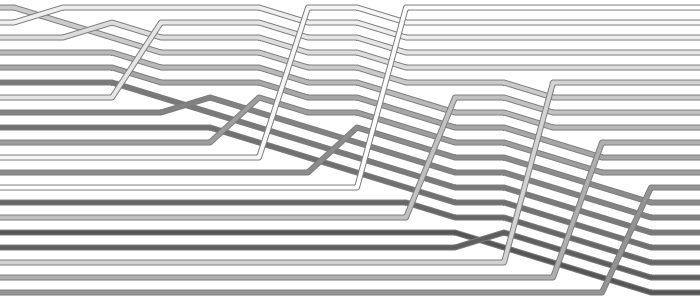
\includegraphics[width=\linewidth]{insertion.png}

%   \centerline{Algorithme A.}
% \end{minipage}\hfill\begin{minipage}{.49\linewidth}
%   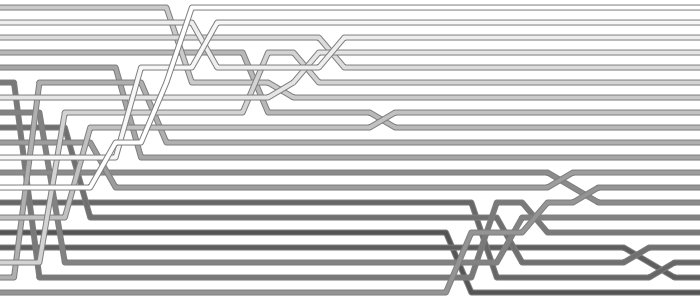
\includegraphics[width=\linewidth]{quick.png}

%   \centerline{Algorithme B.}
% \end{minipage}

% \noindent\begin{minipage}{.49\linewidth}
%   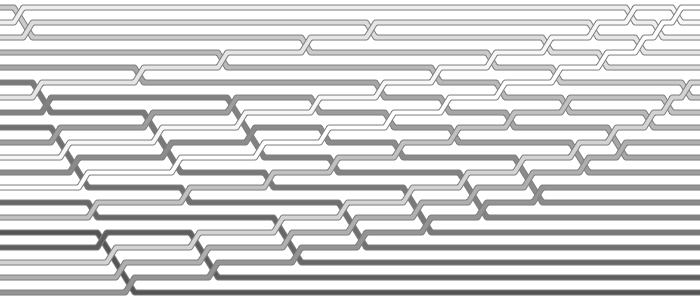
\includegraphics[width=\linewidth]{bubble.png}

%   \centerline{Algorithme C.}
% \end{minipage}\hfill\begin{minipage}{.49\linewidth}
%   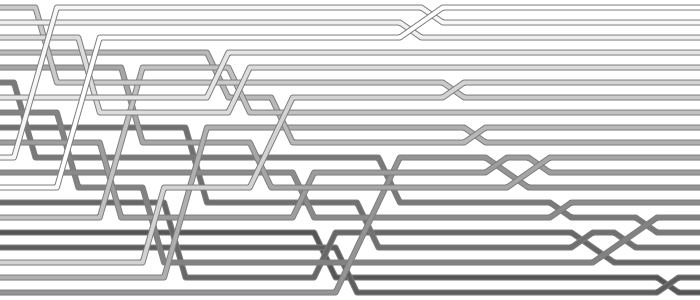
\includegraphics[width=\linewidth]{shell.png}

%   \centerline{Algorithme D.}
% \end{minipage}

% \begin{center}
%   \begin{minipage}{.49\linewidth}
%     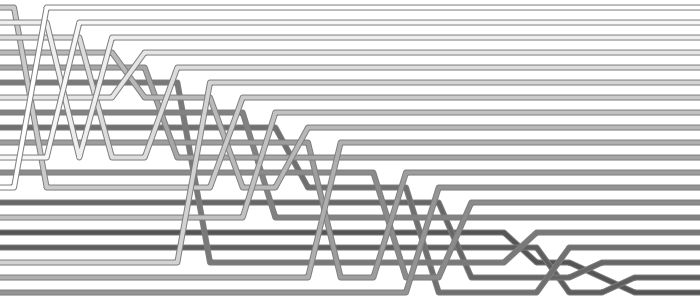
\includegraphics[width=\linewidth]{selection.png}

%     \centerline{Algorithme E.}
%   \end{minipage}
% \end{center}

% \begin{Reponse}
%   \textbf{Tri a bulle:} parcours successifs du tableau en comparant les voisins
%   2 à 2. S'ils sont mal triés, on les inverse. Ce comportement a tendance à
%   pousser les grosses valeurs vers la fin. On peut reconnaitre ce comportement
%   dans l'algorithme C.

%   \textbf{Tri par insertion:} invariant: ce qui est avant la frontière est
%   trié. A chaque étape, je prend l'élément juste après la frontière, et je le
%   met à sa place dans la partie déjà triée. On peut reconnaitre ce comportement
%   dans l'algorithme A.

%   \textbf{Tri par selection:} a chaque étape, je selectionne le minimum de la
%   partie non triée et le pose à la frontière. On reconnait l'algorithme E.

%   \textbf{Shell sort:} comme un bubble sort, mais on commence par trier avec un
%   écartement supérieur à 1. Au lieu d'inverser des voisins, on inverse des
%   cases à distance 3 puis 2 puis on fait un bubble standard, mais sur un
%   tableau un peu prétrié. C'est l'algorithme D.

%   \textbf{Quick sort:} c'est un algorithme récursif qui trie une partie du
%   tableau puis l'autre (les parties ne sont pas forcément de taille
%   identique). C'est l'algorithme B.
% \end{Reponse}

\bigskip
\noindent\hspace{-1.3em}$\bigstar$\textbf{Annexe:} Règles de calcul des
préconditions. 

\begin{itemize}
\item \WP{nop, Q}  $\equiv Q$
\item \WP{x:=E, Q} $\equiv Q[x:=E]$
\item \WP{C;D, Q}  $\equiv$ \WP{C, \WP{D,Q}}
\item \textbf{WP}(\texttt{if} $Cond$ \texttt{then} $C$ \texttt{else} $D$,$Q$)
  $\equiv (Cond=\mathtt{true}\Rightarrow \mathbf{WP}(C,Q))~\wedge~
          (Cond=\mathtt{false}\Rightarrow \mathbf{WP}(D,Q))$
\item \textbf{WP}(\texttt{while} $E$ \texttt{do} $C$ \texttt{done} \{inv I var
  V\},Q)  $\equiv I$ ~~;~~  Obligations de preuve:
  \begin{enumerate}
  \item[$\bullet$] $(E=\mathtt{true}\wedge I\wedge V=z) \Rightarrow
    \mathbf{WP}(C,I\wedge V<z))$
  \item[$\bullet$] $I\Rightarrow V\geq 0$
  \item[$\bullet$] $(E=\mathtt{false}\wedge I) \Rightarrow Q$
  \end{enumerate}
\end{itemize}


\end{document}


%%% Local Variables:
%%% coding: utf-8
